\subsection{Calorimeter Systems}
\label{sec:calorimeters}

The ATLAS calorimeter systems are situated outside of the ID and central solenoid and
are tasked with the measurement and containment of showers from electrically charged and neutral particles.
A view of the calorimeter systems is provided by Figure~\ref{fig:atlas_calorimeters_cutaway}.
Broadly speaking, there are two types of calorimeters based on their purpose:
electromagnetic and hadronic calorimeters.
The electromagnetic calorimeter system has $\eta$ coverage that matches the inner-detector
and is optimized for precision measurements of electrons and photons.
The hadronic calorimeter system has readout cells that are generally of
coarser granularity as compared to the electrogmagnetic calorimeter and
is designed to meet the requirements for jet and missing transverse momentum
measurements.
Besides classification by physics purpose, the calorimeter system can also
be broken into two classes based on detector technology: either based
on gaps of cooled liquid-argon~\cite{CERN-LHCC-96-041} or on scintillating tiles as the active media~\cite{CERN-LHCC-96-042}.

\begin{figure}[!htb]
    \begin{center}
        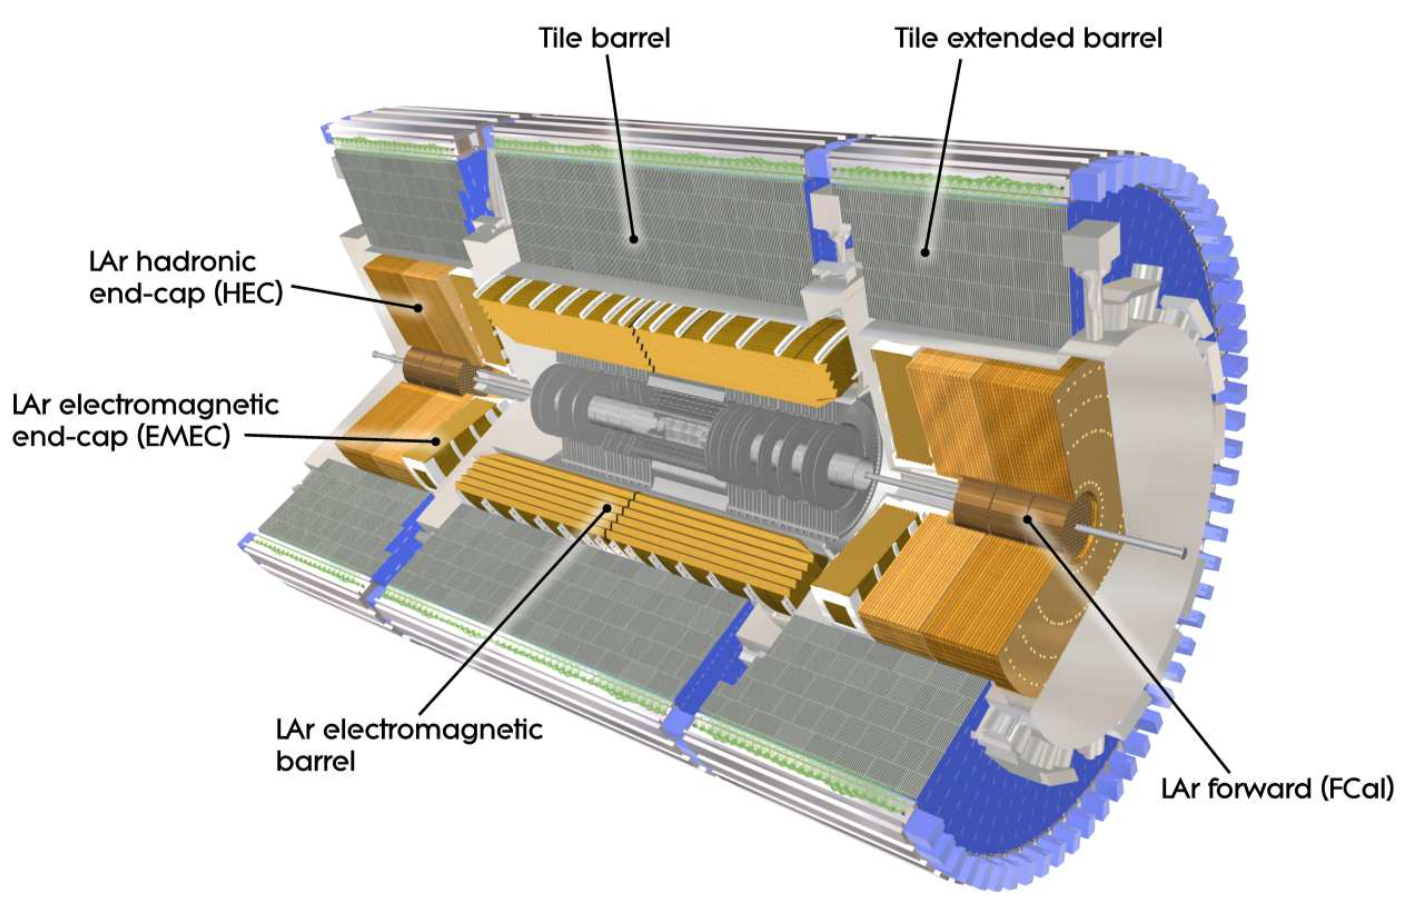
\includegraphics[width=0.9\textwidth]{figures/chapter2/calorimeters/atlas_calorimeter_cutaway}
        \caption{
            Cut-away view of the ATLAS calorimeter system, with liquid-argon and sctintillating-tile
            subsystems indicated.
        }
        \label{fig:atlas_calorimeters_cutaway}
    \end{center}
\end{figure}

\subsubsection{Electromagnetic Calorimeter}
\label{sec:calo_em}

The electromagnetic (EM) calorimeter is a high-granularity lead/liquid-argon (LAr)
sampling calorimeter situated outside of the ID and sharing the
same cryostat as the the central solenoid.
It consists of barrel and end-cap sections that cover the entire
range within $\lvert \eta \rvert < 3.2$ and is illustrated in Figure~\ref{fig:atlas_calorimeters_cutaway}.
The structures of the electromagnetic barrel and end-cap calorimeters
are shown in Figure~\ref{fig:em_calo_section}.
The EM calorimeter is designed in an accordian type structure to provide full coverage
in $\phi$.
The cooled LAr fills the gaps between layers of the
accordian structure.
Passing particles from the interaction point undergo scattering and bremsstrahlung processes as they pass through
the lead absorbers. The resulting electrons and photons ionise the LAr, producing
drift electrons and ions whose signals are read out by the interleaved readout
electrodes. The 2.1\,mm drift gap has an operating voltage of $\approx 2$\,kV.
The electromagnetic calorimeter is $>22$ radiation lengths ($X_0$), ensuring
that the majority of electrons and photons are completely contained within the EM calorimeter.
The majority of the EM energy, amounting to approximately 16\,$X_0$, is contained
within the second sampling layer (see Figure~\ref{fig:em_calo_section}).
The fine granularity of the readout, indicated in Figure~\ref{fig:em_calo_section},
was designed with the ability to distinguish individual photons arising from $\pi^0 \rightarrow \gamma \gamma$
decays. The ability to distinguish photons pairs so precisely is also important for the
main Higgs boson decay channel used for its disovery, $h \rightarrow \gamma \gamma$.

In the region $\lvert \eta \rvert < 1.8$, a so-called \textit{presampler} detector is used to correct
for the energy lost by electrons and photons due to material interactions occuring
upstream of the EM calorimeter.
It is a single LAr layer, with width 1.1\,cm (0.5\,cm) in the barrel (end-cap).

\begin{figure}[!htb]
    \begin{center}
        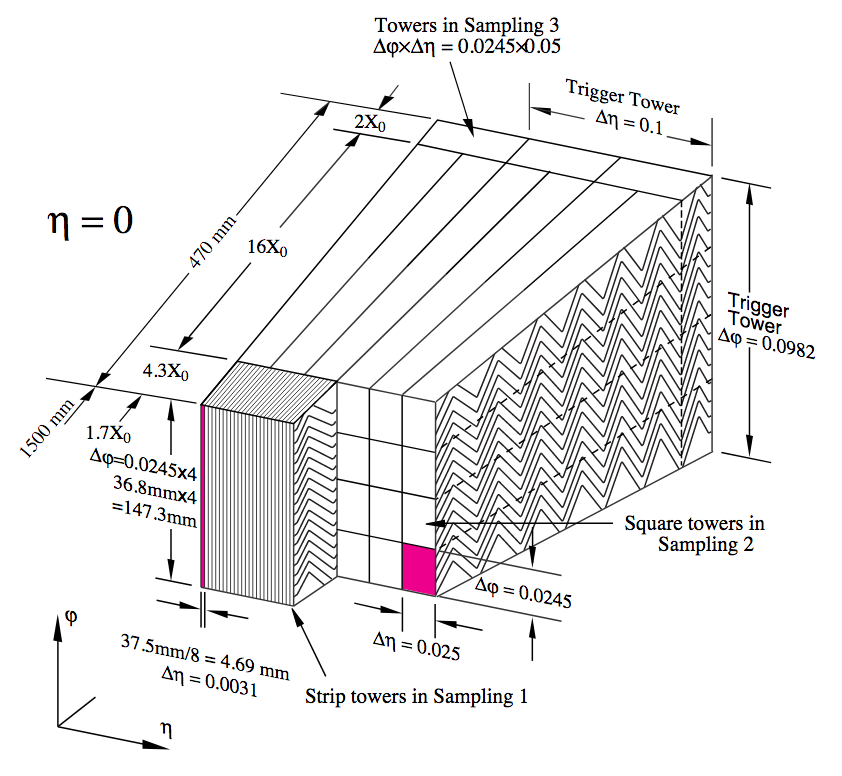
\includegraphics[width=0.6\textwidth]{figures/chapter2/calorimeters/atlas_em_calo_barrel}
        \raisebox{1.5cm}{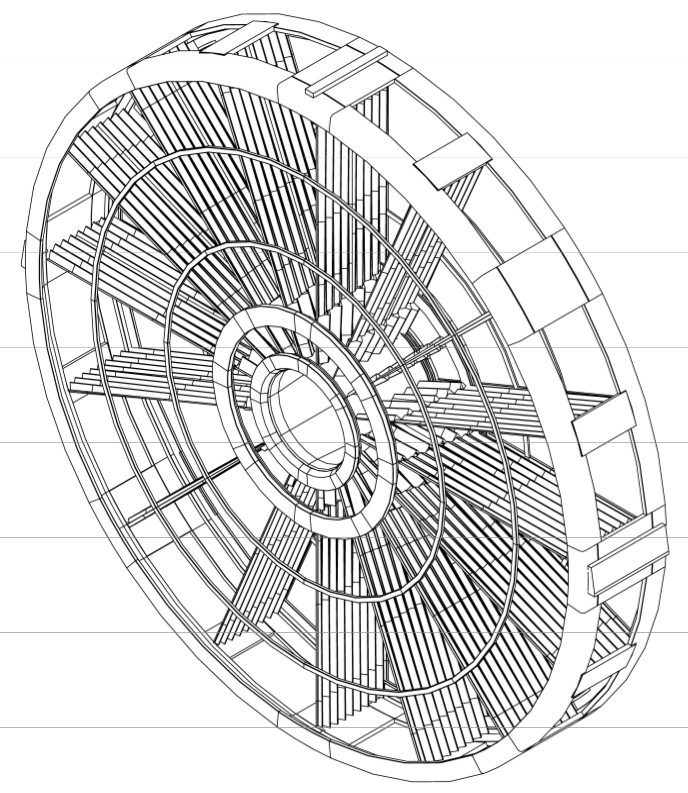
\includegraphics[width=0.3\textwidth]{figures/chapter2/calorimeters/atlas_em_calo_endcap}}
        \caption{
            \textit{Left}: Cut-away view of the barrel electromagnetic calorimeter and its accordian
                structure. Indicated are
                the geometry and absorption properties of the three sampling layers.
                Also indicated is the granularity of the electrode readout in $\Delta \phi \times \Delta \eta$
                in each layer.
            \textit{Right}: Diagram of the electromagnetic end-cap calorimeter accordian wheel structure
                (only a sub-set of the accordian structure is shown).
        }
        \label{fig:em_calo_section}
    \end{center}
\end{figure}

\FloatBarrier
\subsubsection{Hadronic Calorimeter}
\label{sec:calo_had}

The barrel section of the hadronic calorimeter is composed of a
lead/scintillating-tile type detector whereas the end-cap hadronic
calorimeter is based on copper/LAr-based technology.

The lead/scintillating-tile calorimeter (the `tile calorimeter') is located just beyond
the EM calorimeter.
It is composed of a barrel section, covering $\lvert \eta \rvert < 1.0$,
and two extended barrels that cover $0.8 < \lvert \eta \rvert < 1.7$ (see Figure~\ref{fig:atlas_calorimeters_cutaway}).
It is a sampling calorimeter using steel as the passive absorber and scintillating
plastic tiles as the active media.
The tile calorimeter is composed of modules in which the scintillating
tiles are situated in $(r-\phi)$ within the steel absorbers, as shown in Figure~\ref{fig:tile_calo}.
The detector is segmented radially into three layers and the readout of the
scintillation light, using wavelength-shifting fibers that are fed into photomultiplier tubes (PMT)
situated along the outer radii, is organized in a projective
geometry, also illustrated in Figure~\ref{fig:tile_calo}.
In the barrel (extended barrel) section, most of the hadronic energy is captured by the first (last) two
layers which account for $\approx 5.5$ ($6$) hadronic interaction lengths ($\lambda$)
of the $\approx 7$ in total.

The hadronic end-cap (HEC) calorimeter consists of two wheels per end-cap, situated
behind the electromagnetic end-cap calorimeter, and
provides calorimetric coverage in the range $1.5 < \lvert \eta \rvert <3.2$.
A view of the HEC can be seen in Figures~\ref{fig:atlas_calorimeters_cutaway} and \ref{fig:fcal}.
The HEC calorimeter is built from layers of copper plates interleaved with 8.5\,mm LAr gaps
which provide the active medium for this sampling calorimeter.
The readout structure is obtained by dividing the gaps into separate drift zones for
which there are dedicated readout electrodes.
This readout structure is arranged in a projective geometry.

\begin{figure}[!htb]
    \begin{center}
        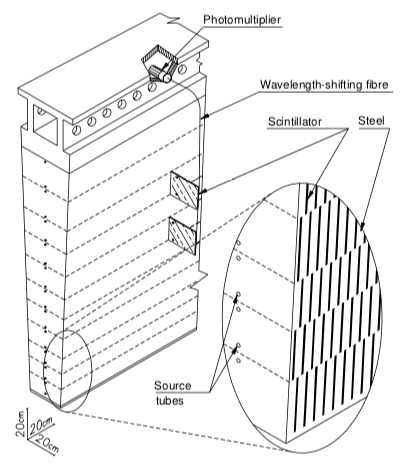
\includegraphics[width=0.4\textwidth]{figures/chapter2/calorimeters/atlas_tile_module}
        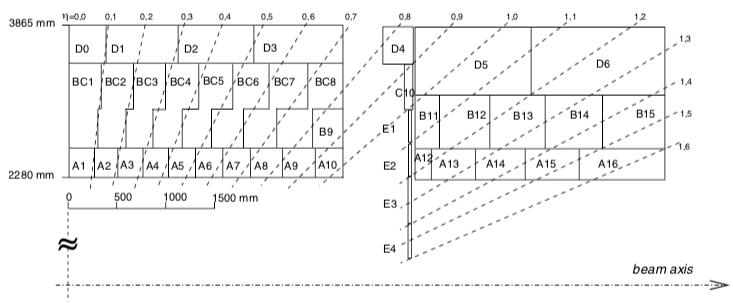
\includegraphics[width=0.9\textwidth]{figures/chapter2/calorimeters/atlas_tile_plan_view}
        \caption{
            \textit{Top}: A view of a tile calorimeter module with its interleaved steel
                absorbers and scintillating tiles and PMT readout. Also indicated are the source tubes
                through which radioactive Cesium (Cs) sources are passed for calibration purposes~\cite{Marjanovic:2018ohl}.
            \textit{Bottom}: Illustration of the segmentation of the projective readout of
                both the barrel and extended barrel tile calorimeter.
        }
        \label{fig:tile_calo}
    \end{center}
\end{figure}

\FloatBarrier
\subsubsection{Forward Calorimeter}
\label{sec:calo_forward}

The forward calorimeter (FCal) system~\cite{Artamonov_2008} provides calorimetric coverage to
high $\lvert \eta \rvert$, between $3.1 < \lvert \eta \rvert < 4.9$,
furthering the hermeticity of the detector.
As indicated in Figure~\ref{fig:fcal}, FCal consists of three layers in the
$z$ direction: an electromagnetic layer (FCal 1) and two hadronic layers (FCal 2 and FCal 3).
All three layers use LAr as the active medium but differ in their passive media.
FCal 1 uses copper for its absorber, chosen for its heat removal properties,
while FCal 2 and FCal 3 use tungsten, chosen to provide high containment and
minimisation of the lateral spread of hadronic showers.
The FCal modules consist of matrices of the passive material with regularly
spaced readout tubes  oriented parallel to the beam-pipe that are filled with the cooled LAr.

\begin{figure}[!htb]
    \begin{center}
        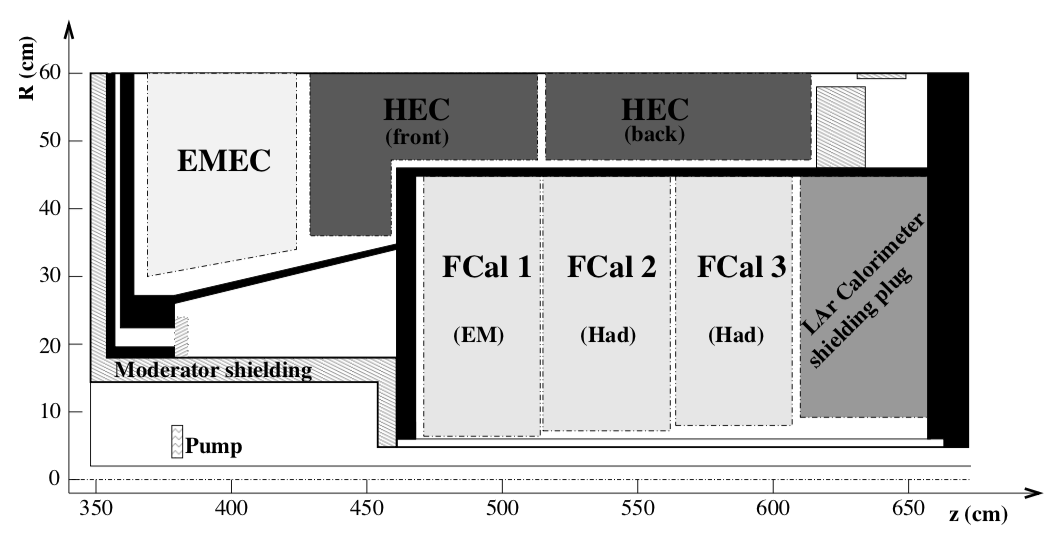
\includegraphics[width=0.65\textwidth]{figures/chapter2/calorimeters/atlas_fcal}
        \caption{
            View of the forward calorimeter (FCal) system. Portions of the electromagnetic
            and hadronic end-cap systems are also shown.
        }
        \label{fig:fcal}
    \end{center}
\end{figure}
